%%%%%%%%%%%%%%%%%%%%%%%%%%%%%%%%%%%%%%%%%%%%%%%%%%%%%%%%%%%%%%%%%%%%%%
%%%%%%%%%%%%%%%%%%%%%%%%%%%%%%%%%%%%%%%%%%%%%%%%%%%%%%%%%%%%%%%%%%%%%%
%%%%                   Relationship arcs
%%%%%%%%%%%%%%%%%%%%%%%%%%%%%%%%%%%%%%%%%%%%%%%%%%%%%%%%%%%%%%%%%%%%%%
%%%%%%%%%%%%%%%%%%%%%%%%%%%%%%%%%%%%%%%%%%%%%%%%%%%%%%%%%%%%%%%%%%%%%%

\section{Relationships}\label{sec:relationships}

\glyph{Relationships} are rules that decide of the existence of entity nodes, based on the existence of others. 
%In ontology parlance, they would be ``occurants''. 
\SBGNERLone{} provides two types of relationships, the statements and the influences.

%%%%%%%%%%%%%%%%%%%%%%%%%%%%%%%%%%%%%%%%%%%%%%%%%%%%%%%%%%%%%%%%%%%%%%
%%%%%%%%%%%%%%%%%%%%%%%%%%%%%%%%%%%%%%%%%%%%%%%%%%%%%%%%%%%%%%%%%%%%%%
%%%%                   Statements
%%%%%%%%%%%%%%%%%%%%%%%%%%%%%%%%%%%%%%%%%%%%%%%%%%%%%%%%%%%%%%%%%%%%%%
%%%%%%%%%%%%%%%%%%%%%%%%%%%%%%%%%%%%%%%%%%%%%%%%%%%%%%%%%%%%%%%%%%%%%%

\subsection{Statements}\label{sec:statements}

\glyph{Statements} can be true or false. \glyph{Statements} are targets of \glyph{Influences}. They are not true themselves, but can  carry \glyph{Outcomes}( see \sect{outcome}). \SBGNERLone{} provides three types of statements, \glyph{Assignment}, \glyph{Interaction} and \glyph{Phenotype}.

%%%%%%%%%%%%%%%%%%%%%%%%%%%%%%%%%%%%%%%%%%%%%%%%%%%%%%%%%%%%%%%%%%%%%%
%%                    Assignment
%%%%%%%%%%%%%%%%%%%%%%%%%%%%%%%%%%%%%%%%%%%%%%%%%%%%%%%%%%%%%%%%%%%%%%

\subsection{Glyph: \glyph{Assignment}}\label{sec:assignment}

\glyph{Assignment} is used to describe the setting of a state variable to a certain value. The assignment, represented by an harpoon arrow, goes from a variable value, represented by a floating \glyph{state variable} to a variable identification, represented by a \glyph{state variable} attached to the entity affected by the assignment.  The result of an assignment is represented by \glyph{outcomes}, that is by filled dots on the arrow. The result of an \glyph{assignment} can be represented by any number of \glyph{outcomes}.

\question{NLN}{The arrowhead of assignment is currently the same than of interactions. It was suggested that we either one or the other or both. But no single combination was really esthetically nice.}

\begin{glyphDescription}
 \glyphSboTerm non-applicable
 \glyphOrigin A state-variable (section \sect{stateVariable}) on its own containing a variable value.
 \glyphTarget A state-variable (section \sect{stateVariable}) carried by a interactor (section \sect{interactors}), containing a variable identification.
 \glyphEndPoint The target extremity of an \glyph{assignment} carries an harpoon arrowhead.
 \end{glyphDescription}

\begin{center}
\scalebox{0.5}{\includegraphics{images/assignment}}
\end{center}
% 
% The following example illustrates the phosphorylation of the protein phosphatase inhibitor DARPP-32 on the threonine 34.
% 
% \begin{center}
% \scalebox{0.5}{\includegraphics{images/assignment-example1.eps}}
% \end{center}
% 
% The following example illustrates two alternative assignments of the state variable ``pore'' or the nAChR. The assignment of the value ``open'' is stimulated by nicotine, while the assignement of the value ``desens'' (desensitised) is stimulated by curare. 
% 
% \begin{center}
% \scalebox{0.5}{\includegraphics{images/assignment-example2.eps}}
% \end{center}

\normalcolor

\newpage
%%%%%%%%%%%%%%%%%%%%%%%%%%%%%%%%%%%%%%%%%%%%%%%%%%%%%%%%%%%%%%%%%%%%%%
%%                    Interaction
%%%%%%%%%%%%%%%%%%%%%%%%%%%%%%%%%%%%%%%%%%%%%%%%%%%%%%%%%%%%%%%%%%%%%%
\color{blue}

\subsection{Glyph: \glyph{Interaction}}\label{sec:interaction}

\glyph{Interaction} represents an interaction between two \glyph{entity} or \glyph{outcome}, whether non-covalent physical interaction, or functional interaction, e.g. genetic interaction. Each arrowhead points to an interactor involved in the interaction. The result of the interaction is represented by \glyph{outcomes} (see section \ref{sec:outcome}), that is by filled dots on the line linking the two arrowheads. The result of an interaction can be represented by any number of \glyph{outcomes}.

\begin{glyphDescription}
 \glyphSboTerm SBO:0000342 molecular or genetic interaction
 \glyphOrigin \glyph{entity} \sect{entity} or \glyph{outcome} \sect{outcome}.
 \glyphTarget \glyph{entity} \sect{entity} or \glyph{outcome} \sect{outcome}.
 \glyphEndPoint Both origin and target extremities of an \glyph{interaction} carry an harpoon arrowhead.
 \end{glyphDescription}

\begin{center}
\scalebox{0.5}{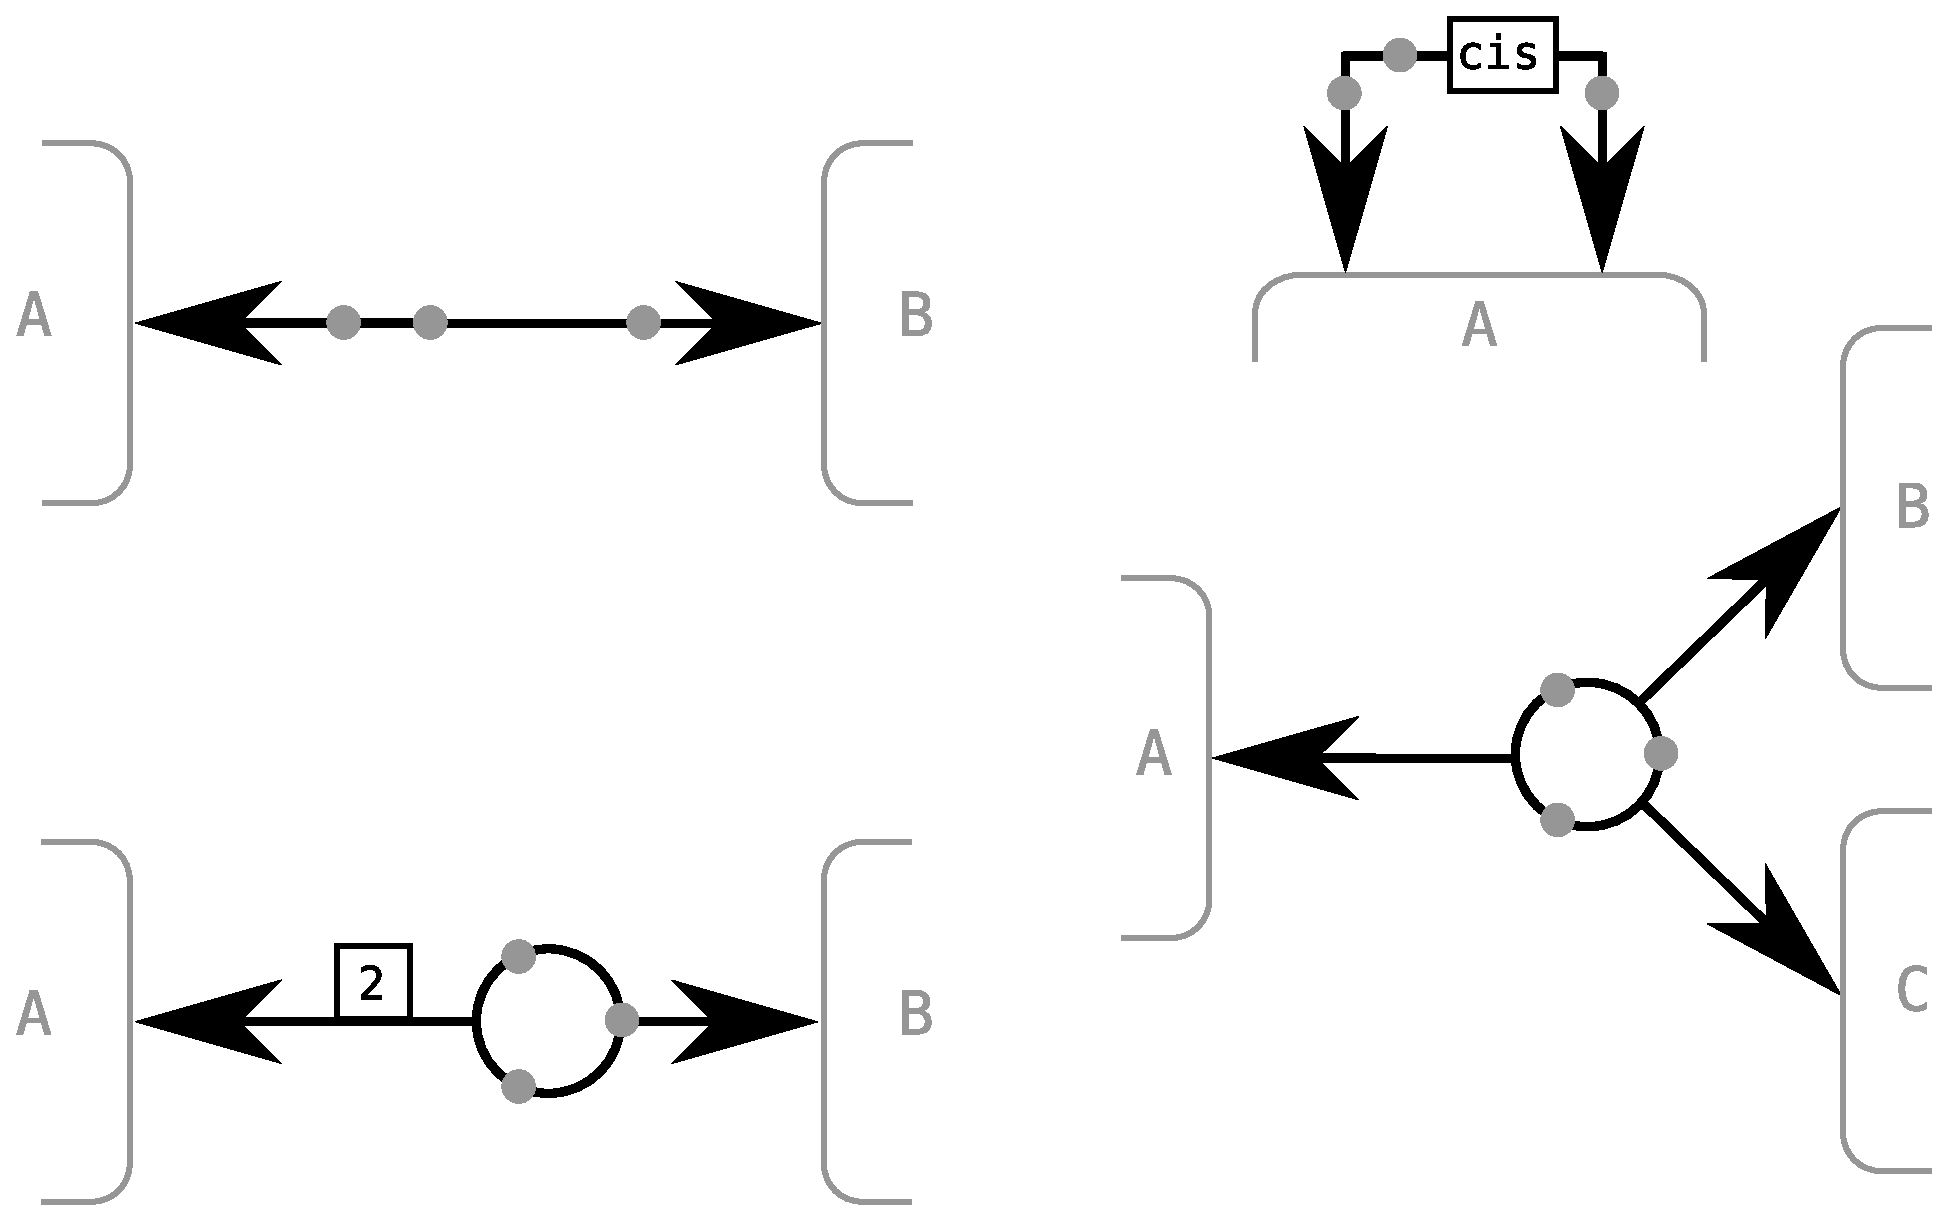
\includegraphics{images/interaction}}
\end{center}

\question{NLN}{TREAT THE CASE OF NON-BINARY INTERACTIONS}

 
% The following example illustrates the interaction of cyclin and CDC2 kinase to form the Maturation Promoting Factor in ER.
% 
% \begin{center}
% \scalebox{0.5}{\includegraphics{images/interaction-example1.eps}}
% \end{center}
\normalcolor

\newpage

\color{ForestGreen}

\subsection{Glyph: \glyph{Phenotype}}
\label{sec:phenotype}

A biochemical network can generate phenotypes or affect biological
processes.  Such processes can take place at different levels and are
independent of the biochemical network itself.  To represent these
processes in a diagram, SBGN defines the \glyph{phenotype} glyph.

\begin{glyphDescription}

\glyphSboTerm SBO:0000358 ! phenotype
\glyphOrigin Non-applicable
\glyphTarget Non-applicable
\glyphEndPoint A \glyph{phenotype} is represented by an elongated
hexagon, as illustrated in \fig{phenotype}. It is identified by a label placed in an
unbordered box containing a string of characters.  The characters can be
distributed on several lines to improve readability, although this is not
mandatory.  The label box must be attached to the center of the
\glyph{phenotype} container.  The label may spill outside of the container.

\end{glyphDescription}
 
\begin{figure}[H]
  \centering
  \includegraphics[scale = 0.3]{images/phenotype}
  \caption{The \ER glyph for \glyph{phenotype}.}
  \label{fig:phenotype}
\end{figure}

\begin{figure}[H]
  \centering
  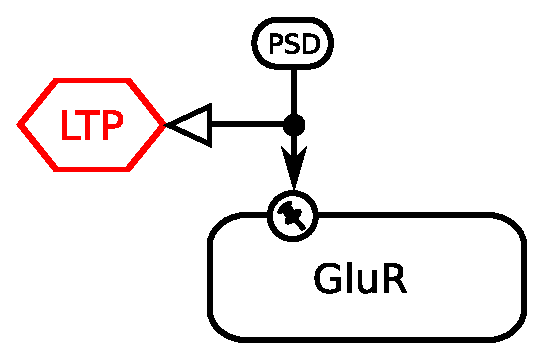
\includegraphics[scale = 0.5]{examples/ex-phenotype}
  \caption{Example of a \glyph{phenotype} ``Long Term Potentiation (LTP)'' enhanced when the entity ``GluR'' is present in the post-synaptic density.}
  \label{fig:ex-phenotype}
\end{figure}

\normalcolor


\subsection{Influences}\label{sec:influences}

Influence arcs represent the effect of an entity on another relationship. The symbols attached to their extremities precise their semantics. SBGN \ERs{}' influences can be viewed as logical rules linking \glyph{ENs} and other rules. \SBGNERLone{} provides seven influences, \glyph{Modulation}, \glyph{Stimulation}, \glyph{Inhibition}, \glyph{Necessary Stimulation}, \glyph{Absolute Inhibition}, \glyph{Absolute Stimulation}, \glyph{Logic Arc}.

%%%%%%%%%%%%%%%%%%%%%%%%%%%%%%%%%%%%%%%%%%%%%%%%%%%%%%%%%%%%%%%%%%%%%%
%%                     Modulation
%%%%%%%%%%%%%%%%%%%%%%%%%%%%%%%%%%%%%%%%%%%%%%%%%%%%%%%%%%%%%%%%%%%%%%
%\color{blue}
\subsubsection{Glyph: \glyph{Modulation}}\label{sec:modulation}

A \glyph{modulation} affects the propensity, or the chances to happen, of the target relationship. Such a modulation can affect the relationship \textbf{positively or negatively}, or even both ways depending on the conditions. A \glyph{modulation} can also be used when one does not know the precise direction of the effect, for instance if there are conflicting evidences.

\begin{glyphDescription}
 \glyphSboTerm SBO:0000168 ! control.
 \glyphOrigin Any \glyph{entity node} (\sect{ENs}).
 \glyphTarget Any \glyph{relationship} (\sect{relationships}).
 \glyphEndPoint The target extremity of a \glyph{modulation} carries an empty diamond.
 \glyphAux A \glyph{unit of information} carrying the mention \glyph{cis} or \glyph{trans} precises the relationship between the \glyph{entity node} from which the \glyph{modulation} origins and either:
\begin{itemize}
\item the \glyph{entity node} from which the influence targeted by the \glyph{modulation} origins
\item all the relevant \glyph{interactors} of the \glyph{interaction} targeted by the \glyph{modulation}
\item the \glyph{entity} subjected to the \glyph{assignment} targeted by the \glyph{modulation}
\end{itemize}
 \end{glyphDescription}

\begin{figure}[H]
  \centering
  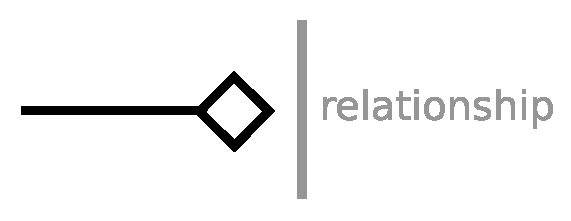
\includegraphics[scale = 0.5]{images/modulation}
  \caption{The \ER glyph for \glyph{modulation}.}
  \label{fig:modulation}
\end{figure}
 
% \begin{figure}[H]
%   \centering
%   \includegraphics[scale = 0.5]{examples/ex-modulation}
%   \caption{Example of a \glyph{modulation} of the \glyph{phenotype} ``Long Term Potentiation (LTP)'' by the phosphorylation of an \glyph{entity} ``target''. For instance the influence could be positive (stimulation, see \sect{stimulation}) or negative (inhibition, see \sect{inhibition}).}
%   \label{fig:ex-modulation}
% \end{figure}

%\normalcolor


%%%%%%%%%%%%%%%%%%%%%%%%%%%%%%%%%%%%%%%%%%%%%%%%%%%%%%%%%%%%%%%%%%%%%%
%%                     Stimulation
%%%%%%%%%%%%%%%%%%%%%%%%%%%%%%%%%%%%%%%%%%%%%%%%%%%%%%%%%%%%%%%%%%%%%%

\subsection{Glyph: \glyph{Stimulation}}\label{sec:stimulation}
\color{blue}

A stimulation affects \textbf{positively} the the strength, or the probability, of the target relationship. This stimulation can be for instance a catalysis or a positive allosteric regulation.

\begin{glyphDescription}
 \glyphSboTerm SBO:0000170 ! stimulation.
 \glyphOrigin Any \glyph{interactor} (\sect{interactors}) or any \glyph{logical operator} (\sect{logic}).
 \glyphTarget Any \glyph{relationship} (\sect{relationships}).
 \glyphEndPoint The target extremity of a \glyph{stimulation} carries an empty arrowhead.
 \end{glyphDescription}

\begin{figure}[H]
  \centering
  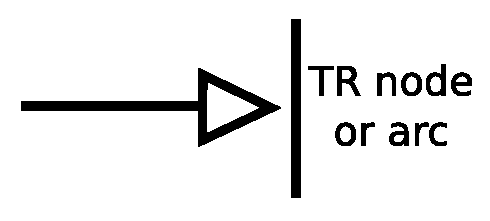
\includegraphics[scale = 0.5]{images/stimulation}
  \caption{The \PD glyph for \glyph{stimulation}.}
  \label{fig:stimulation}
\end{figure}



%%%%%%%%%%%%%%%%%%%%%%%%%%%%%%%%%%%%%%%%%%%%%%%%%%%%%%%%%%%%%%%%%%%%%%
%%                     Inhibition
%%%%%%%%%%%%%%%%%%%%%%%%%%%%%%%%%%%%%%%%%%%%%%%%%%%%%%%%%%%%%%%%%%%%%%

\subsubsection{Glyph: \glyph{Inhibition}}\label{sec:inhibition}
%\color{blue}

An \glyph{inhibition} affects \textbf{negatively}  the strength, or the probability, of the target relationship. This inhibition can be for instance a steric hindrance or a negative allosteric regulation.

\begin{glyphDescription}
 \glyphSboTerm SBO:0000170 ! inhibition.
 \glyphOrigin Any \glyph{entity node} (\sect{ENs}).
 \glyphTarget Any \glyph{relationship} (\sect{relationships}).
 \glyphEndPoint The target extremity of a \glyph{inhibition} carries a bar perpendicular to the arc.
 \glyphAux A \glyph{unit of information} carrying the mention \glyph{cis} or \glyph{trans} precises the relationship between the \glyph{entity node} from which the \glyph{inhibition} origins and either:
\begin{itemize}
\item the \glyph{entity node} from which the influence targeted by the \glyph{inhibition} origins
\item all the relevant \glyph{interactors} of the \glyph{interaction} targeted by the \glyph{inhibition}
\item the \glyph{entity} subjected to the \glyph{assignment} targeted by the \glyph{inhibition}
\end{itemize}
 \end{glyphDescription}

\begin{figure}[H]
  \centering
  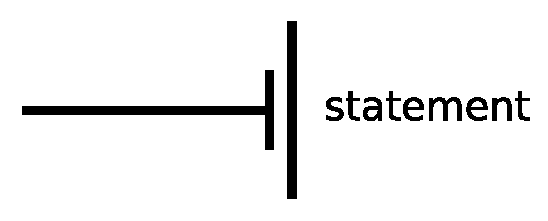
\includegraphics[scale = 0.5]{images/inhibition}
  \caption{The \ER glyph for \glyph{inhibition}.}
  \label{fig:inhibition}
\end{figure}

\begin{figure}[H]
  \centering
  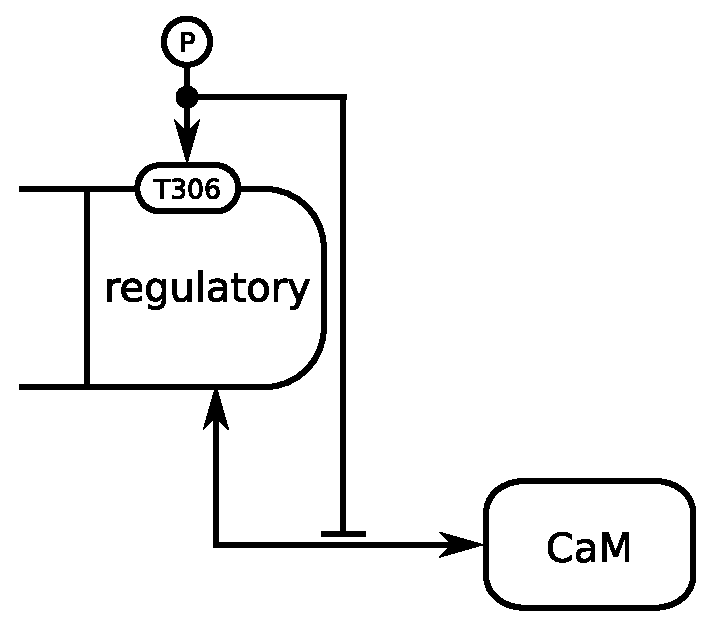
\includegraphics[scale = 0.5]{examples/ex-inhibition}
  \caption{In this example, the phosphorylation of the threonine 306 of the regulatory domain of CaMKII inhibits the interaction between Calmodulin and the kinase.}
  \label{fig:ex-inhibition}
\end{figure}

%\normalcolor


%%%%%%%%%%%%%%%%%%%%%%%%%%%%%%%%%%%%%%%%%%%%%%%%%%%%%%%%%%%%%%%%%%%%%%
%%                     necessary stimulation
%%%%%%%%%%%%%%%%%%%%%%%%%%%%%%%%%%%%%%%%%%%%%%%%%%%%%%%%%%%%%%%%%%%%%%
%\color{blue}

\subsubsection{Glyph: \glyph{Necessary stimulation}}\label{sec:necessaryStimulation}

A \glyph{necessary stimulation} is an influence that has to be present for a relationship to take place (to become true). A relationship modulated by a necessary stimulation can only exist when this stimulation is true, whatever are the other influences this relationship is subjected to.

\begin{glyphDescription}
 \glyphSboTerm SBO:0000171 ! necessary stimulation.
 \glyphOrigin Any \glyph{entity node} (\sect{ENs}).
 \glyphTarget Any \glyph{relationship} (\sect{relationships}).
 \glyphEndPoint The target extremity of a \glyph{necessary stimulation} carries an open arrow (to remind that it is a \glyph{stimulation}) coming after a larger vertical bar.
 \glyphAux A \glyph{unit of information} carrying the mention \glyph{cis} or \glyph{trans} precises the relationship between the \glyph{entity node} from which the \glyph{necessary stimulation} origins and either:
\begin{itemize}
\item the \glyph{entity node} from which the influence targeted by the \glyph{necessary stimulation} origins
\item all the relevant \glyph{interactors} of the \glyph{interaction} targeted by the \glyph{necessary stimulation}
\item the \glyph{entity} subjected to the \glyph{assignment} targeted by the \glyph{necessary stimulation}
\end{itemize}

 \end{glyphDescription}

\begin{figure}[H]
  \centering
  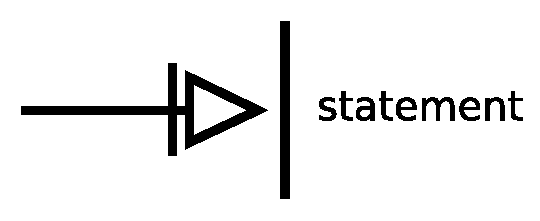
\includegraphics[scale = 0.5]{images/necessaryStimulation}
  \caption{The \ER glyph for \glyph{necessary stimulation}.}
  \label{fig:necessaryStimulation}
\end{figure}

\begin{figure}[H]
  \centering
  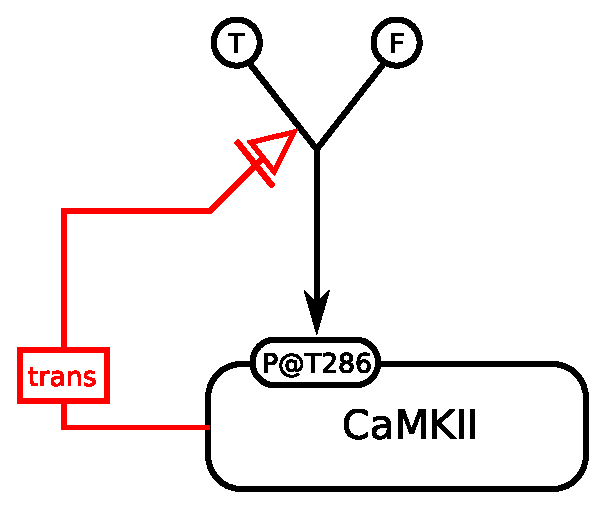
\includegraphics[scale = 0.5]{examples/ex-necessaryStimulation}
  \caption{This example shows how threonine 286 of CaMKII is only phosphorylated by the kinase itself, but in a trans-fashion, meaning a molecule of CaMKII does not phosphorylate itself, but another molecule of CaMKII.}
  \label{fig:ex-necessaryStimulation}
\end{figure}

%\normalcolor
%%%%%%%%%%%%%%%%%%%%%%%%%%%%%%%%%%%%%%%%%%%%%%%%%%%%%%%%%%%%%%%%%%%%%%
%%                     absolute stimulation
%%%%%%%%%%%%%%%%%%%%%%%%%%%%%%%%%%%%%%%%%%%%%%%%%%%%%%%%%%%%%%%%%%%%%%
%\color{blue}

\subsubsection{Glyph: \glyph{Absolute inhibition}}\label{sec:absoluteInhibition}

An \glyph{absolute inhibition} precludes the existence of another relationship. A relationship modulated by an absolute inhibition can only exist when an absolute inhibition in false, whatever are the other influences this relationship is subjected to.

\begin{glyphDescription}
 \glyphSboTerm SBO:0000407 ! absolute inhibition.
 \glyphOrigin Any \glyph{entity node} (\sect{ENs}).
 \glyphTarget Any \glyph{relationship} (\sect{relationships}).
 \glyphEndPoint The target extremity of a \glyph{absolute inhibition} carries a double bar perpendicular to the arc (to remind that it is an \glyph{inhibition}).
\begin{itemize}
\item the \glyph{entity node} from which the influence targeted by the \glyph{absolute inhibition} origins
\item all the relevant \glyph{interactors} of the \glyph{interaction} targeted by the \glyph{absolute inhibition}
\item the \glyph{entity} subjected to the \glyph{assignment} targeted by the \glyph{absolute inhibition}
\end{itemize}

 \end{glyphDescription}

\begin{figure}[H]
  \centering
  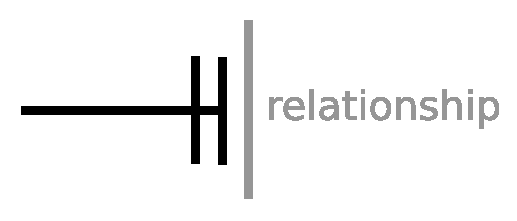
\includegraphics[scale = 0.5]{images/absoluteInhibition}
  \caption{The \ER glyph for \glyph{absoluteInhibition}.}
  \label{fig:absoluteInhibition}
\end{figure}

\begin{figure}[H]
  \centering
  \includegraphics[scale = 0.5]{examples/ex-absoluteInhibition}
  \caption{This example shows how an intra-molecular interaction of CaMKII precludes totally its catalytic activity upon another molecule of CaMKII.}
  \label{fig:ex-absoluteInhibition}
\end{figure}

%\normalcolor
%%%%%%%%%%%%%%%%%%%%%%%%%%%%%%%%%%%%%%%%%%%%%%%%%%%%%%%%%%%%%%%%%%%%%%
%%                     absolute stimulation
%%%%%%%%%%%%%%%%%%%%%%%%%%%%%%%%%%%%%%%%%%%%%%%%%%%%%%%%%%%%%%%%%%%%%%
%\color{red}

\subsubsection{Glyph: \glyph{Absolute stimulation}}\label{sec:absoluteStimulation}

An absolute stimulation always triggers the existence of a target relationship. 

\begin{glyphDescription}
 \glyphSboTerm SBO:0000411 ! absolute stimulation
 \glyphOrigin Any \glyph{entity node} (\sect{ENs}).
 \glyphTarget Any \glyph{relationship} (\sect{relationships}).
 \glyphEndPoint The target extremity of \corr{a}{an} \glyph{absolute stimulation} carries a double empty arrowhead (to remind that it is a \glyph{stimulation}).
 \glyphAux A \glyph{unit of information} carrying the mention \glyph{cis} or \glyph{trans} precises the relationship between the \glyph{entity node} from which the \glyph{absolute stimulation} origins and either:
\begin{itemize}
\item the \glyph{entity node} from which the influence targeted by the \glyph{absolute stimulation} origins
\item all the relevant \glyph{interactors} of the \glyph{interaction} targeted by the \glyph{absolute stimulation}
\item the \glyph{entity} subjected to the \glyph{assignment} targeted by the \glyph{absolute stimulation}
\end{itemize}
 \end{glyphDescription}

\begin{figure}[H]
  \centering
  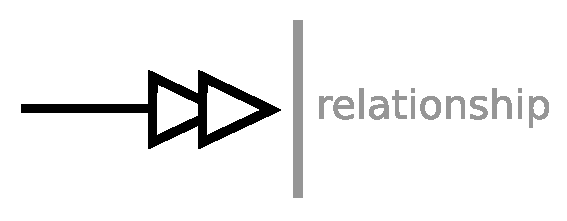
\includegraphics[scale = 0.5]{images/absoluteStimulation}
  \caption{The \ER glyph for \glyph{absolute stimulation}.}
  \label{fig:absoluteStimulation}
\end{figure}

%\normalcolor

%%%%%%%%%%%%%%%%%%%%%%%%%%%%%%%%%%%%%%%%%%%%%%%%%%%%%%%%%%%%%%%%%%%%%%
%%                     Logic arc
%%%%%%%%%%%%%%%%%%%%%%%%%%%%%%%%%%%%%%%%%%%%%%%%%%%%%%%%%%%%%%%%%%%%%%
\color{blue}
\subsubsection{Glyph: \glyph{Logic arc} }\label{sec:logicArc}

\glyph{Logic arc} is used to represent the fact that an interactor influences
the outcome of a logic operator. 

\begin{glyphDescription}
 \glyphSboTerm SBO:0000398 - logical relationship.
 \glyphOrigin Any \glyph{interactor} (\sect{interactors}) or \glyph{logical operator} (\sect{logic}).
 \glyphTarget Any \glyph{logical operator} (\sect{logic}).
 \glyphEndPoint No particular symbol is used to represent a logic arc.
 \end{glyphDescription}

\begin{figure}[H]
  \centering
  
\includegraphics[scale = 0.4]{images/logicArc}
  \caption{The \ER glyph for \glyph{logic arc}.}
  \label{fig:logicArc}
\end{figure}

\begin{figure}[H]
  \centering
  \includegraphics[scale = 0.5]{examples/ex-logicArc}
  \caption{In this example, two logic arcs reflect the fact that the intra-molecular interaction of either the cis- or trans-subunits of CaMKII precludes the phosphorylation of threonine 286 by the trans-subunit.}
  \label{fig:ex-logicArc}
\end{figure}

\normalcolor

%\section{Submap}\label{sec:submap}
%% $HeadURL: https://sbgn.svn.sourceforge.net/svnroot/sbgn/trunk/documents/specifications/EntityRelationship/Level1/sources/submap.tex $
\color{red}
\section{Glyph: \glyph{Submap}}
\label{sec:submap}

A \glyph{submap} is used to encapsulate entities and relationships (including all types of nodes and edges) within one glyph.  

TO BE FILLED.


\normalcolor

% The following is for [X]Emacs users.  Please leave in place.
% Local Variables:
% TeX-master: "../sbgn_ER-level1"
% End:



